% Joshua Reed
% Fall, 2017
% 
% hw2_chpt_2.tex
% 
% Homework for random processes.

\documentclass[12pt]{article}
\usepackage[margin=1in]{geometry} 
\usepackage{amsmath,amsthm,amssymb}
\usepackage{listings}
\usepackage[compact]{titlesec}
\usepackage{graphicx}
\graphicspath{{img/}}
%\usepackage{enumitem}
\usepackage{enumerate}
\usepackage{float}

\setlength\parindent{0cm}
\setlength\parskip{0.2cm}
\raggedright{}
\newcommand{\mysection}[1]{\section*{#1}}


\begin{document}
{\large \bfseries %Header section
  Joshua Reed\\
  Fall, 2017 \\
  \centering
  {\huge Homework 2 Chapter 2}\\
  EE 520 Random Processes \\
  Problems: 2.3, 2.7, 2.9, 2.10, 2.19, 2.22, 2.28, 2.30, 2.31, and 2.38}
 
 
\mysection{2.3} 
In a restaurant known for its unusual service, the time X, in minutes, that a customer has to wait
before he captures the attention of a waiter is specified by the following.


\begin{equation*}
  F_X(x)=\
    \begin{cases}
      {(\frac{x}{2})}^2, & \text{for }0\leq x \leq1,\\
      \frac{x}{4}, & \text{for }1\leq x \leq2,\\
      \frac{1}{2}, & \text{for }2\leq x \leq10,\\
      \frac{x}{20}, & \text{for }10\leq x \leq20,\\
      1, & \text{for }x\geq 20,
    \end{cases}
\end{equation*}


\begin{enumerate}[(a)]
  \item 
    Sketch $F_x(x)$.
    \begin{figure}[H]\centering
      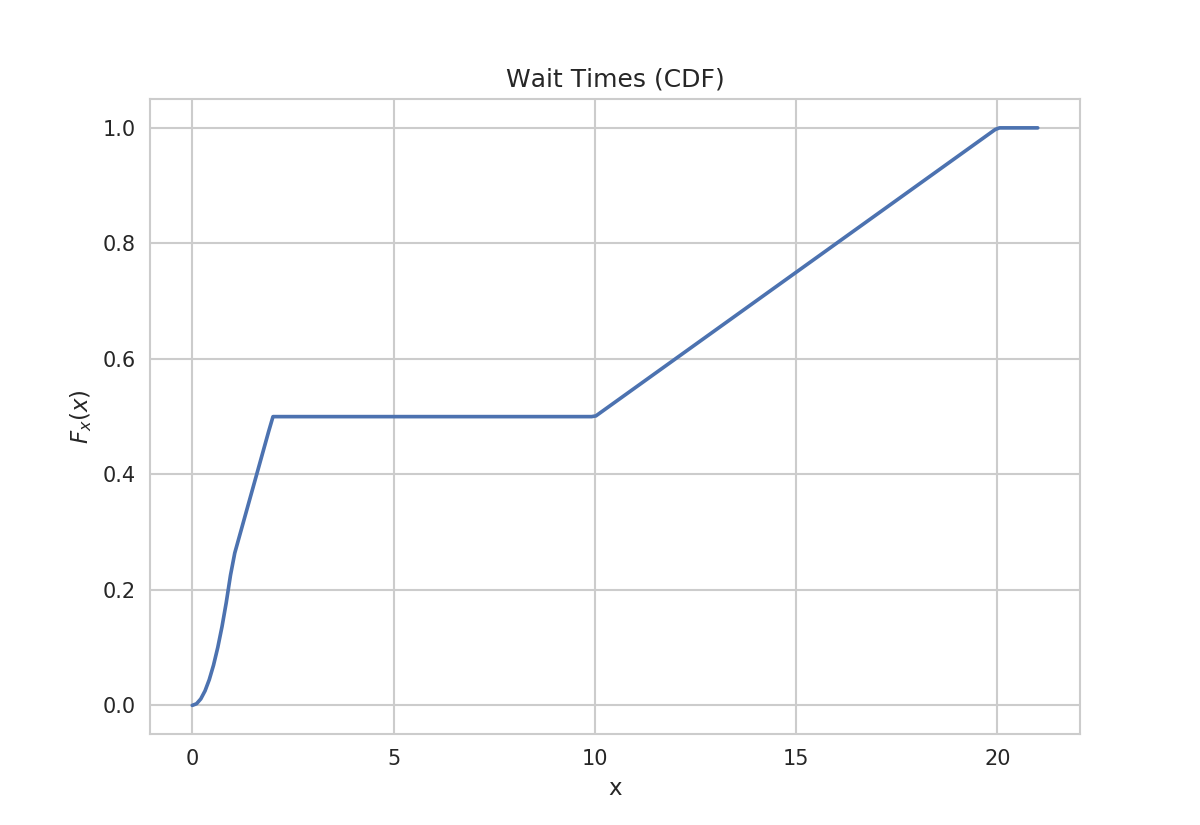
\includegraphics[scale=0.7]{plot-wait-times-cdf}
    \end{figure}
    \newpage
    
  \item 
    Compute and sketch the PDF $f_x(x)$
    
    The PDF is the differential of the CDF, so the derivative of $F_x(X)$ will be the PDF $f_x(x)$.
    
    For this problem, I am assuming that $F_x(x)$ is piecewise differentiable.\\
    \begin{align*}
    \frac{d}{dx}({(\frac{x}{2})}^2) &= \frac{d}{dx}(\frac{x^2}{4})\\
    &= 2\frac{x}{4}\\
    &= \frac{x}{2}
    \end{align*}
    
    \begin{align*}
    \frac{d}{dx}(\frac{x}{4}) &= \frac{1}{4}
    \end{align*}
    
    \begin{align*}
    \frac{d}{dx}(\frac{1}{2}) &= 0
    \end{align*}
    
    \begin{align*}
    \frac{d}{dx}(\frac{x}{20}) &= \frac{1}{20}
    \end{align*}
    
    \begin{equation*}
      F_X(x)=\
        \begin{cases}
          \frac{x}{2}, & \text{for }0\leq x \leq1,\\
          \frac{1}{4},  & \text{for }1\leq x \leq2,\\
          0,            & \text{for }2\leq x \leq10,\\
          \frac{1}{20}, & \text{for }10\leq x \leq20,\\
          0,            & \text{for }x\geq 20,
        \end{cases}
    \end{equation*}
    
    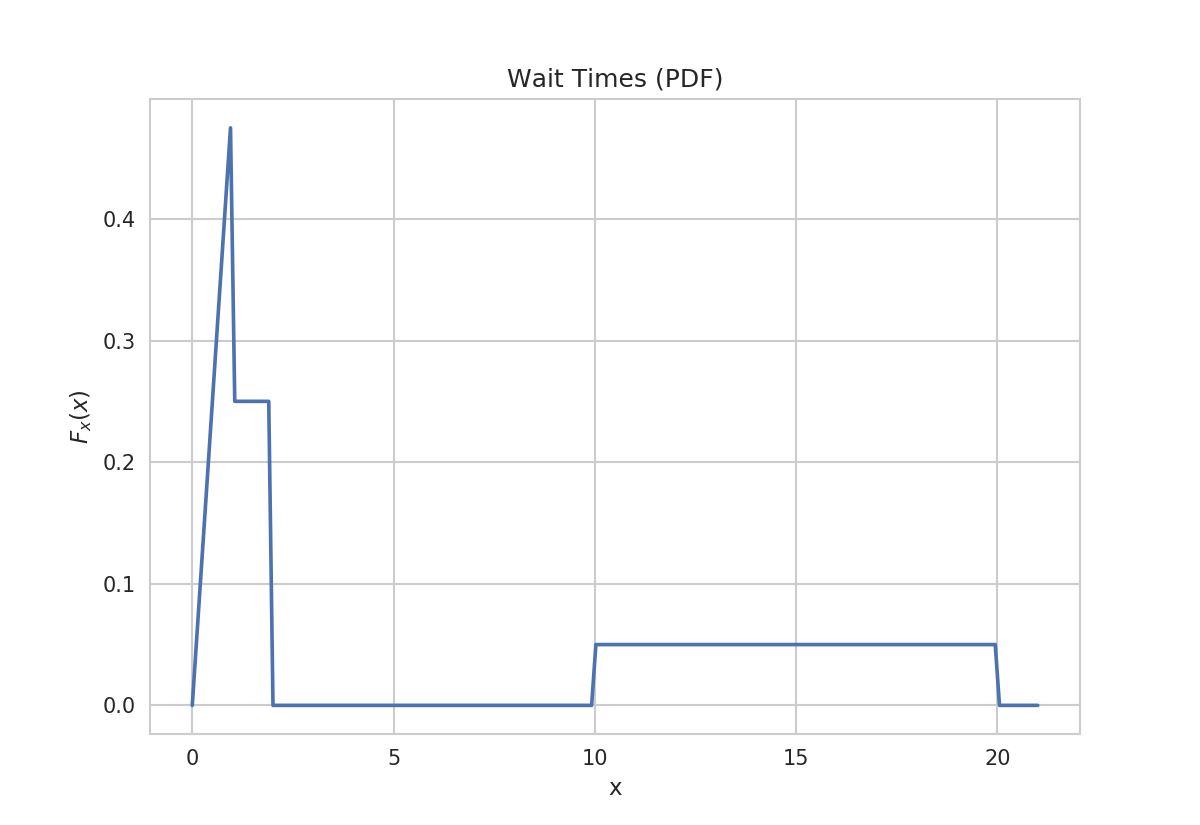
\includegraphics[scale=0.7]{plot-wait-times-pdf}

  \item
    What is the probability that the customer will have to wait (1) at least 
    10 minutes, (2) less than 5 minutes, (3) between 5 and 10 minutes, (4) exactly 1 minute?
    
    \begin{enumerate}[(1)]  
      \item $P(X\geq10)=P(x\leq \infty)-P(x\leq10)=F_x(20)-F_x(10)=1-1/2=1/2$
      \item $P(X\leq5)=F_x(5)=1/2$
      \item $P(5\leq x \leq 10)=P(x\leq 10) -P(x\leq5)=1/2-1/2=0$
      \item $P(x=1)=f_x(1)=$ either 1/2, 1/4, or more plausably 0.
    \end{enumerate}
    
    Because the likelihood of being served at \emph{exactly} 1 minute is zero.

\end{enumerate}
\newpage



\mysection{2.7} 
A noisy resistor produces a voltage $v_n(t)$. At $t=t_1$, the noise level 
$X\stackrel{\Delta}{=}v_n(t_1)$ is known to be a Gaussian RV with PDF\\

  \[ f_X(x)=\frac{1}{\sqrt{2\pi\sigma^2}}e^{-\frac{1}{2}{(\frac{x}{\sigma})}^2} \]

Compute and plot the probability that $|X|>k\sigma$ for $k=1,2,\ldots$
\begin{figure}\centering
  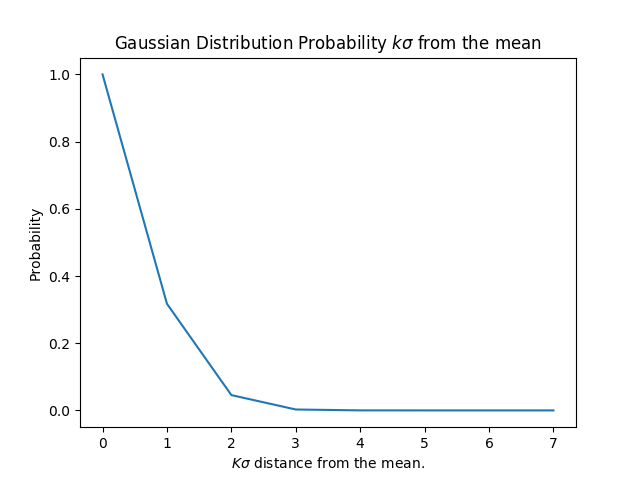
\includegraphics[scale=0.7]{plot_gaussian_ksigma}
\end{figure}
\newpage




\mysection{2.9}
Write PDFs using $\delta$ functions for the Bernoulli binomial, and Poisson PMF's.
\begin{itemize}
  \item Bernoulli \\
    With probability of success p.
    \begin{align*}
      f_X(x)&=
      \begin{cases}
        p^x{(1-p)}^{1-x},  & \text{for } x=0, 1 \\
        0, & \text{for all others}
      \end{cases}\\
      &=\delta(x-1)p+\delta(x)(1-p)
    \end{align*}

  \item Binomial \\
    \[ P[X=k]=\binom{n}{k}p^k{(1-p)}^{n-k} \]
    \[ f_X(x)=\sum_{k=0}^n \delta(x-k) \binom{n}{k}p^k{(1-p)}^{n-k} \]
    
  \item Poisson \\
    \[ P[X=k]=\frac{{(\lambda t)}^k}{k!}e^{-\lambda t} \]
    \[ f_X(x)=\sum_{k=0}^\infty \delta(x-k) \frac{{(\lambda t)}^k}{k!}e^{-\lambda t} \]
\end{itemize}
\newpage







\mysection{2.10}
The PDF of a RV X is shown in figure P2.10. The numbers in the parenthesis indicate area. 
\begin{enumerate}[(a)]
  \item Compute the value of A.
    \begin{align*}
      1&=\int_1^4 Ae^{-x} dx + \int_1^4 1/4[\delta(x-2)+\delta(x-3)] dx\\
       &=A[(-1)e^{-x}]\big|_1^4 +0.5\\
      \frac{1}{2} &=A[-e^{-4}+e]\\ 
      \frac{1}{2} &=A(0.350)\\ 
       A&=\frac{1}{0.70}\\ 
       A&=1.429
    \end{align*}
  \item Sketch the CDF.\@
    \begin{figure}[H]\centering
      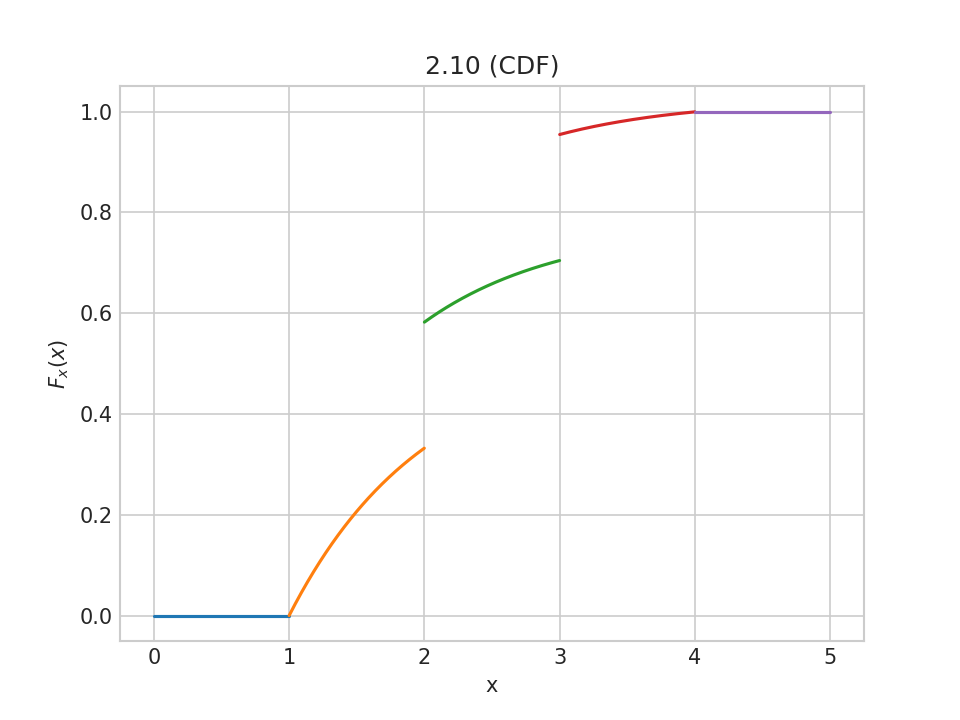
\includegraphics[scale=0.6]{plot_CDF_210}
    \end{figure}
  \item Compute $P[2\leq X<3]$
    From the CDF 
    \begin{align*}
      P[2\leq X<3]&=P[X\leq3]-P[X\leq2]\\
                  &=F_X^-(3)-F_X^-(2)\\
                  &=0.372
    \end{align*} 
  \item Compute $P[2<X\leq 3]$
    The same but with the jump at 3 included instead. \\
    $0.372$

  \item Compute $F_x(3)$.\\
    Here I used python to calculate the value, but it's simply $\int_1^3Ae^{-x}dx+1/2$.
    \[ F_X(3)=0.955 \]
\end{enumerate}
\newpage







\mysection{2.19}
It has been found that the number of people Y waiting in a queue in the bank on payday obeys the Poisson 
law as
\begin{align*}
  P[Y=k|X=x]=e^{-x}\frac{x^k}{k!}, k\geq0, x>0
\end{align*}
Given that the normalized serviing time of the teller x is constant. However, the 
serving time is more accurately modeled as an RV X. For simplicity let X be a uniform RV with 
\begin{align*}
  f_X(x)=\frac{1}{5}[u(x)-u(x-5)]
\end{align*}
Then $P[Y=k|X=x]$ is still Poisson but $P[Y=k]$ is something else. Compute $P[Y=k]$ for $k=0,1, $ 
and $2$. The answer for general k may be difficult.


\begin{align*}
  P[Y=k] &=\int_\infty^\infty P[Y=k|X=x]f_X(x)dx\\
         &=\int_\infty^\infty \frac{x^k}{k!}e^{-x} \frac{1}{5}(u(x)-u(x-5))dx\\
         &=\frac{1}{5}\int_0^5 \frac{x^k}{k!}e^{-x}dx\\
\end{align*}

From here I simply solved numerically in python.

\begin{enumerate}[k=1]
  \item 
    0.199
  \item 
    0.192
  \item 
    0.175
\end{enumerate}

\newpage




\mysection{2.22}
Consider the joint PDF of X and Y:\\
\begin{align*}
f_{XY}(x,y)=\frac{1}{3\pi}e^{-\frac{1}{2}[{(x/3)}^2+{(y/2)}^2]}u(x)u(y)
\end{align*}
\begin{enumerate}
  \item Are X and Y independent RVs?  \\
    Yes, X and Y are independent RVs.
    \begin{align*}
      f_{XY}(x,y)&=\frac{1}{3\pi}e^{-\frac{1}{2}{(\frac{X}{3})}^2}u(x)
                                 e^{-\frac{1}{2}{(\frac{y}{2})}^2}u(y)\\
    \end{align*}
  Here, $\frac{1}{3\pi}$ is the equivalent of $\frac{C}{2\pi \sigma_x \sigma_y}$ and $\sigma_x = 3$, $\sigma_y = 2$
  \begin{align*}
    \frac{1}{3\pi}&=\frac{C}{2\pi\sigma_X\sigma_Y}\\
                  &=\frac{C}{2\pi(3)(2)}\\
                  &=\frac{C}{\pi12}
  \end{align*}
  \begin{align*}
    C_{12}&=\frac{12}{3}\\
          &=4
  \end{align*}
  Thus $C_1$ and $C_2 = 2$.

  And finally, 
  \[ f_X(x)=\frac{2}{\sqrt{2\pi}3}e^{-{\frac{1}{2}(\frac{x}{3})}^2} \text{,\quad and \quad} 
     f_Y(y)=\frac{2}{\sqrt{2\pi}2}e^{-{\frac{1}{2}(\frac{y}{2})}^2} \]

  \item Compute the probability of $\{0<X\leq3, 0<Y\leq2\}$.
    \[ erf(x)=\frac{2}{\sqrt\pi}\int_0^x e^{-x^2}dx \]
    \begin{align*}
      P[\{0<X\leq3,\ 0<Y\leq2\}]&=\int_0^2\int_0^3 f_X(x)f_Y(y) dx\ dy\\
                               &=F_X(3)F_Y(2)\\
                               &=\frac{1}{3}erf(\frac{x}{3\sqrt2})\frac{1}{2}erf(\frac{y}{2\sqrt2})\\
                               &=\frac{1}{3}erf(\frac{3}{3\sqrt2})\frac{1}{2}erf(\frac{2}{2\sqrt2})\\
                               &=erf(\frac{1}{\sqrt2})erf(\frac{1}{\sqrt2})\\
                               &=0.466
    \end{align*}
\end{enumerate}
\newpage 




\mysection{2.28}
Let $X$ be a random variable with a PDF of 
\begin{align*}
  f_X(x) =
  \begin{cases}
    0,          &\ x< 0,\\
    ce^{-2x},   &\ x\geq 0,
  \end{cases}
\end{align*}
  for, $c>0$.
\begin{enumerate}[(a)]
  \item Find c  \\
    The pdf must integrate to 1.

    \begin{align*}
      F_X(\infty)&=c\int_0^\infty e^{-2x}dx = 1\\
                 &=c\frac{-1}{2}e^{-2x}\big|_0^\infty\\
                 &=c\frac{1}{2}\\
                c&=2
    \end{align*}
  
  \item Let $a>0$, $x>0$, find $P[X\geq x+a]$
    \begin{align*}
      P[X\geq x+a]&=\int_{x+a}^\infty2e^{-2x}dx\\
                  &=-e^{-2x}\big|_{x+a}^\infty\\
                  &=e^{-2(x+a)}
    \end{align*}

  \item Let $a>0$, $x>0$, find $P[X\geq x+a|X\geq a]$
    \begin{align*}
      P[X\geq x+a|X>a]&=\frac{P[(X\geq x+a)\cap(X\geq a)]}{P[X\geq a]}\\
                      &=\frac{e^{-2(x+a)}}{e^{-2a}}\\
                      &=e^{-2x}
    \end{align*}
\end{enumerate}
\newpage 




\mysection{2.30}
A U.S. defense radar scans the skies for unidentified flying objects (UFOs). Let $M$ be the event that a UFO is
present and $M^c$ the event that the UFO is absent. Let 
$f_{X|M}(x|M)=\frac{1}{\sqrt{2\pi}}e^{-\frac{1}{2}{(x-r)}^2}$ be the conditional pdf of the radar return
signal X when a UFO is actually there, and let 
$f_{X|M^c}=\frac{1}{\sqrt{2\pi}}e^{-\frac{1}{2}{(x)}^2}$ be the conditional pdf of the radar return signal X
when there is no UFO\@. To be specific, let $r=1$ and let the alert level be $x_A=1/2$. Let A denote the event
of an alert, that is ${X>x_a}$. \\
Here, 
  \[ P[A]=P[X>1/2]=\int_{1/2}^\infty f_X(x) dx \]
  \[ f_X(x)=f_{X|M^c}(x)P[M^c]+f_{X|M}(x)P[M] \]
Compute
\begin{enumerate}
  \item $P[A|M]=$\\
    Here the $P[M]=1$
    \begin{align*}
      P[A|M]&=\int_{1/2}^\infty f_{X|M}(x) dx\\
            &=\int_{1/2}^\infty \frac{1}{\sqrt{2\pi}}e^{-\frac{1}{2}{(x-r)}^2} dx\\
            &=\int_{1/2}^\infty \frac{1}{\sqrt{2\pi}}e^{-\frac{1}{2}{(x-1)}^2} dx\\
            &=0.691
    \end{align*}
  \item $P[A^c|M]$\\
    \begin{align*}
      P[A^c|M]&=\int_{0}^{1/2} f_{X|M}(x) dx\\
            &=\int_{0}^{1/2} \frac{1}{\sqrt{2\pi}}e^{-\frac{1}{2}{(x-r)}^2} dx\\
            &=0.309
    \end{align*}
  \item $P[A|M^c]$\\
    \begin{align*}
      P[A|M^c]&=\int_{1/2}^\infty f_{X|M}(x) dx\\
            &=\int_{1/2}^\infty \frac{1}{\sqrt{2\pi}}e^{-\frac{1}{2}{(x)}^2} dx\\
            &=0.309
    \end{align*}
  \item $P[A^c|M^c]$\\
    \begin{align*}
      P[A^c|M^c]&=1-P[A|M^c]\\
            &=0.691
    \end{align*}
\end{enumerate}
\newpage




\mysection{2.31}
In the previous problem assume that $P[M]=10^-3$. Compute

  \[ P[M|A],P[M|A^c],P[M^c|A],P[M^c|A^c]\text{. Repeat for } P[M]=10^-6 \]

  \begin{align*}
    P[A]&=P[A|M]P[M]+P[A|M^c]P[M^c]
        &=0.691(10^-3)+0.309(1-10^-3)
        &=0.3089
  \end{align*}

\begin{enumerate}
  \item $P[M|A]$\\
    \begin{align*}
      P[M|A]&=\frac{P[M\cap A]}{P[A]}\\
            &=\frac{0.691(10^-3)}{0.3089}\\
            &=0.00224
    \end{align*}
  \item $P[M^c|A]$\\
    \begin{align*}
      P[M^c|A]&=1-P[M|A]\\
              &=0.998
    \end{align*}
  \item $P[M|A^c]$\\
    \begin{align*}
      P[M^c|A]&=\frac{P[M^c\cap A]}{1-P[A]}\\
            &=\frac{0.3085(10^-3)}{0.6911}\\
            &=0.000446
    \end{align*}
  \item $P[M^c|A^c]$\\
    \begin{align*}
      P[M^c|A]&=1-P[M|A^c]\\
            &=0.9996
    \end{align*}
\end{enumerate}
\newpage

And again with $P[M]=10^-6$.

  \begin{align*}
    P[A]&=P[A|M]P[M]+P[A|M^c]P[M^c]
        &=0.691(10^-6)+0.309(1-10^-6)
        &=0.3085
  \end{align*}

\begin{enumerate}
  \item $P[M|A]$\\
    \begin{align*}
      P[M|A]&=\frac{P[M\cap A]}{P[A]}\\
            &=\frac{0.691(10^-6)}{0.3089}\\
            &=0.000224
    \end{align*}
  \item $P[M^c|A]$\\
    \begin{align*}
      P[M^c|A]&=1-P[M|A]\\
              &=0.999998
    \end{align*}
  \item $P[M|A^c]$\\
    \begin{align*}
      P[M^c|A]&=\frac{P[M^c\cap A]}{1-P[A]}\\
            &=\frac{0.3085(10^-6)}{0.6911}\\
            &=0.0000446
    \end{align*}
  \item $P[M^c|A^c]$\\
    \begin{align*}
      P[M^c|A]&=1-P[M|A^c]\\
            &=0.9999996
    \end{align*}
\end{enumerate}
\newpage


\mysection{2.38}
A laser used to scan the bar code on supermarket items is assumed to have a constant conditional failure
rate of $\lambda(>0)$. What is the maximum value of $\lambda$ that will yield a probability of a first
breakdown in $100$ hours of operation less than or equal to $0.05$?

Because $\lambda$ is constant, it can be assumed that $F_X(x)=1-e^{-\lambda t}u(t)$

\begin{align*}
  P[X\leq100]&\leq 0.005 \\
  F_X(100)&=1-e^{-\lambda 100}\\
  0.95&\leq e^{-\lambda 100}\\
  \ln{(0.95)}&\leq \ln(e^{-\lambda 100})\\
 -0.0513&\leq -\lambda 100\\
 \lambda 100 &\leq 0.0513\\
 \lambda &\leq \frac{0.0513}{100}\\
 \lambda &\leq 0.000513
\end{align*}

  Here the solution says it should be negative, but I believe it actually should not. 

  The solutions at one point write $\frac{-\ln(0.95)}{100}=-0.000513$, but $\ln(0.95)=-0.05129$.
\newpage


\end{document}
